\documentclass[a4paper]{article}
\usepackage[margin=20mm]{geometry}
\usepackage{amsmath,graphicx,booktabs}
\usepackage[hidelinks]{hyperref}

\title{Classical and Quantum-Assisted Search for QOBLIB Portfolio Optimization}
\author{Quantum Icing Team}
\date{}

\begin{document}
\maketitle

\begin{abstract}
We minimize QOBLIB's multiperiod portfolio objective using exact dynamic programming (DP), classical local
search, and quantum large-neighborhood search with Pauli correlation encoding (PCE).
Across two classical campaigns, six independently obtained 50-asset portfolios improve published best-known
objectives. A search that combines day-level tabu moves with exact asset-trajectory DP finds the two largest
improvements, 61.79\% and 60.33\%. On ten assets, exact DP confirms 64 optima, and three PCE search chains
reach their respective optima using at most nine simulated qubits.
\end{abstract}

\section{Problem formulation}

In QOBLIB's model~\cite{qoblib}, for each period \(t=0,\ldots,T-1\) and asset \(i=1,\ldots,n\), the decision consists of long and short holdings
\(L_{ti},S_{ti}\in\{0,1,2,3\}\). Set \(v_t=L_t-S_t\). The benchmark counts units of holdings, with a limit \(B\)
per period and a capital register \(C=10\). Its constraints are
\begin{equation}
\label{eq:constraints}
\sum_i(L_{ti}+S_{ti})\le B,\qquad
0\le C-\sum_i v_{ti}\le15 .
\end{equation}
The selected ten- and fifty-asset instances use \(B=4\) and \(B=20\), respectively.

The objective combines risk, return, cash interest, short holding fees, and transaction costs.
Let \(R_t(\lambda)\), \(r_t\), \(c_t\), and \(h_t\) be the benchmark's integer-rounded risk, return, transaction,
and short-fee coefficients. With \(C=10\), cash interest contributes \(-10(C-\sum_i v_{ti})\) per period.
Writing the objective in the benchmark's units gives
\begin{equation}
\label{eq:objective}
\begin{aligned}
F(L,S)={}&\sum_{t=0}^{T-1}
\left[v_t^\mathsf{T}R_t(\lambda)v_t+h_t^\mathsf{T}S_t
      -10\left(C-\sum_i v_{ti}\right)\right]
-\sum_{t=0}^{T-2}r_t^\mathsf{T}v_t\\
&+c_0^\mathsf{T}(L_0+S_0)+c_{T-1}^\mathsf{T}(L_{T-1}+S_{T-1})\\
&+\sum_{t=1}^{T-2}c_t^\mathsf{T}
\left(|L_t-L_{t-1}|+|S_t-S_{t-1}|\right).
\end{aligned}
\end{equation}
The separate final-period charge follows the official scorer. We minimize \(F\).
Risk coefficients are rounded after multiplication by \(\lambda\), using the benchmark's rounding convention.
Consequently, the integer coefficient tables must be rebuilt for each risk weight.

\section{Exact dynamic programming on ten assets}

Holding both a long and a short position in the same asset is dominated. Replacing each pair by its net holding
preserves return, risk, and capital, decreases the number of open units, and cannot increase the holding or transaction costs.
We therefore enumerate net holdings \(v\in\{-3,\ldots,3\}^{n}\) subject to \(\sum_i|v_i|\le B\).
For \(n=10,B=4\), this gives 8,341 feasible period states. The capital constraint is automatic because
\(-4\le\sum_i v_i\le4\).

Let \(g_t(v)\) include the costs of holding \(v\) in period \(t\), including any initial or final charge.
The cost of changing holdings is kept separate. Define \(w_t=c_t\)
for \(1\le t\le T-2\) and \(w_{T-1}=0\). The recurrence is
\begin{equation}
\label{eq:dp}
D_0(v)=g_0(v),\qquad
D_t(v)=g_t(v)+\min_{u\in\mathcal V}
\left[D_{t-1}(u)+w_t^\mathsf{T}|v-u|\right].
\end{equation}
Backtracking from \(\min_v D_{T-1}(v)\) recovers the full portfolio.
The implementation sorts predecessor costs so a transition evaluation can stop once its accumulated cost
cannot improve the current minimum.

We reran \eqref{eq:dp} for eight ten-asset instances, covering ten or fifteen periods and four market-data variants,
at each of the eight benchmark risk weights. All 64 objectives match the published reference values.
QOBLIB labels 14 of these references optimal. For the other 50, our optimality classification follows
from the exhaustive state enumeration and exact recurrence, with each recovered portfolio checked by the referee.

\clearpage
\section{Classical search beyond ten assets}

\subsection{Candidate pools and exact neighborhood search}

As the number of assets grows, enumerating every feasible period state becomes expensive.
Our earlier solver builds a pool of candidate holdings from rounded continuous relaxations, descent over single
and paired unit moves, iterated local search, and simulated annealing. During pool construction, it explores
several approximations to entry and exit costs by charging zero, one, or two times the period's transaction
coefficient. It then uses \eqref{eq:dp} to choose a sequence from that pool with the original transaction costs.
This step optimizes the sequence over the pool, so its quality depends on the available holdings.

Large-neighborhood search (LNS) refines the resulting portfolio by fixing all but \(k\le4\) assets and optimizing
those \(k\) trajectories jointly over the full horizon. Each day has at most \(7^k\) candidate states.
The fixed holdings determine the remaining budget and capital constraints, and the risk calculation includes
their interactions with the free assets. We discard infeasible states and solve the restricted problem by DP.

\subsection{Asset-trajectory DP and day-level tabu search}

The new solver starts from a full portfolio and alternates between two views of it.
In the first, one or two assets can change across all days. Exact DP solves these subproblems over 7 or 49
states per day, respectively. Descent sweeps across single assets, then pairs, and keeps improvements.
Iterated local search (ILS) perturbs the portfolio by changing holdings over a random interval of days and then
repeats descent. It can keep an equally good result and periodically returns to the best portfolio found.

In the second view, every asset can change on one day while neighboring days are fixed. The tabu search scans
feasible one-unit changes to one asset or a pair. For a change \(\delta\) to the day's net holdings \(v_t\),
the risk contribution changes by
\[
\delta^\mathsf{T}(R_t+R_t^\mathsf{T})v_t+\delta^\mathsf{T}R_t\delta .
\]
Maintaining \((R_t+R_t^\mathsf{T})v_t\) makes each candidate's risk change inexpensive to evaluate.
The move score also includes fees, cash interest, and rebalancing costs on either side of the day.
The best admissible move can temporarily increase the objective. Reversing a recent move is blocked for
several iterations unless the reversal produces a new best. We restore the best daily holdings and apply trajectory
descent again. On 50 assets with \(B=20\), a daily search uses 250 iterations and a base tabu tenure of nine,
with a random extension. Some daily searches start by clearing the holdings on that day.

These daily moves help build hedges involving several assets. At high \(\lambda\), changing one or two assets
from an empty day may increase risk too much to be accepted by descent. A sequence of such moves can reach a
combination that reduces total cost. In the two largest improvements in Table~\ref{tab:classical},
each day with open positions uses 19 or 20 units across 14--18 assets.

\subsection{Parallel tempering and campaign settings}

Parallel tempering (PT) runs 12 copies of the search at geometrically spaced temperatures. Each copy proposes
block changes over intervals of days and uses a Metropolis acceptance rule. Adjacent temperatures can exchange
portfolios. About every ten seconds within a PT phase, the solver applies trajectory descent to the best
portfolio seen by PT and offers the result to the coldest replica.
The campaign cycles through ILS, day-level tabu search, and PT, sharing the best portfolio between phases.
It used seed 11 and budgets of 45, 120, and 180 seconds per configuration at 10, 50, and 200--400 assets,
respectively.

\clearpage
\section{Classical results}

The 125 archived files cover 56 ten-asset, 56 fifty-asset, and 13 larger configurations.
The 56 ten-asset objectives match their references and agree with the exact DP.
Of the 56 fifty-asset configurations, six raw scores fall below their published best-known value (BKV),
34 match it, and 16 are above it. One of the six improvements starts from the published reference.
Table~\ref{tab:classical} tracks the independent results across the two campaigns.

\begin{table}[htbp]
\centering
\caption{Independent fifty-asset results below a published BKV, all with \(B=20\).
Names omit \texttt{po\_a050\_}. Bold marks the lower team score, used to compute the reduction
\((F_{\rm ref}-F)/|F_{\rm ref}|\).}
\label{tab:classical}
\begin{tabular}{@{}llrrrr@{}}
\toprule
Instance & \(\lambda\) & Published BKV & Earlier best & New campaign & Reduction\\
\midrule
\texttt{t15\_orig} & \(10^{-2}\) & \(-31{,}504\) & \(-45{,}031\) & \textbf{-50,971} & 61.792\%\\
\texttt{t10\_s00} & \(10^{-2}\) & \(-12{,}340\) & \(-17{,}675\) & \textbf{-19,785} & 60.332\%\\
\texttt{t10\_s02} & \(10^{-2}\) & \(-43{,}565\) & \textbf{-45,069} & \(-44{,}625\) & 3.452\%\\
\texttt{t15\_s02} & \(10^{-2}\) & \(-40{,}622\) & \textbf{-41,517} & \(-39{,}998\) & 2.203\%\\
\texttt{t10\_s00} & \(5\cdot10^{-4}\) & \(-234{,}259\) & \(-234{,}587\) & \textbf{-234,696} & 0.187\%\\
\texttt{t15\_s02} & \(5\cdot10^{-4}\) & \(-392{,}668\) & \(-391{,}667\) & \textbf{-392,723} & 0.014\%\\
\bottomrule
\end{tabular}
\end{table}

\begin{figure}[htbp]
\centering
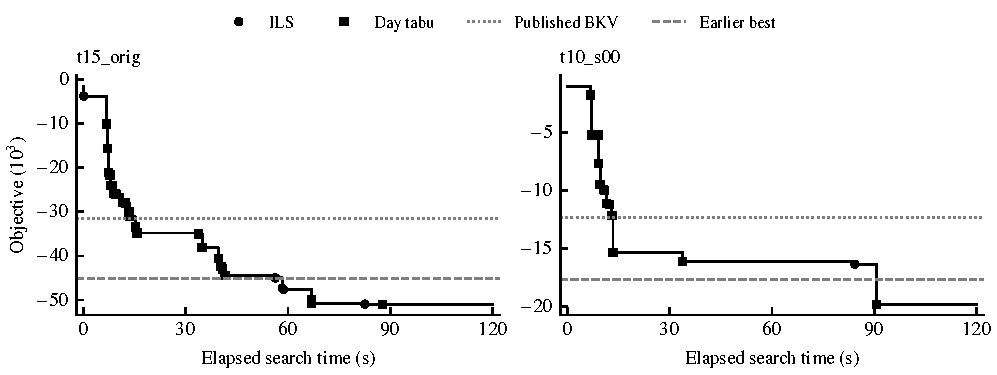
\includegraphics[width=\linewidth]{figures/portfolio-classical-progress.pdf}
\caption{Incumbent objectives for the two largest reductions in Table~\ref{tab:classical}.
Both runs start from empty holdings at \(\lambda=10^{-2}\). Markers identify which phase produced each improvement.
Horizontal lines mark the published BKV and the team's earlier best.}
\label{fig:classical}
\end{figure}

The day-level tabu phase found the two largest gains at 87.7 and 90.7 seconds, respectively
(Figure~\ref{fig:classical}). It also found \(-392{,}723\) at 94.5 seconds, beating the previous
\texttt{t15\_s02} reference at \(\lambda=5\cdot10^{-4}\) by 55 units. At \(\lambda=10^{-2}\) across the eight
50-asset logs, tabu phases produced 93 incumbent improvements, ILS phases 11, and PT phases two.
Each phase received a different time budget and inherited the other phases' progress, so these counts describe
the observed search history. Two scores from the earlier pool-and-LNS method remain the team best.

The separate \texttt{t10\_orig} run at \(\lambda=10^{-2}\) refines QOBLIB's published portfolio from
\(-37{,}107\) to \(-44{,}208\). A separate three-minute run starting from empty holdings reached \(-34{,}853\).
The refinement is recorded in the campaign archive and is excluded from the independent comparison.

The larger runs cover 200 assets with \(B=50\) and 400 with \(B=100\). For instance, the
400-asset, 15-day case at \(\lambda=10^{-3}\) scores \(-2{,}986{,}716\). Its full notebook QUBO would have
36,165 binary variables. The search works with integer net holdings and uses zero qubits.
Published reference values for these configurations are unavailable.

\clearpage
\section{Quantum large-neighborhood search}

\subsection{Compact portfolio QUBO}

The quantum search encodes holdings with three unary copies for each asset, direction, and period.
For example \(L_{ti}=\sum_{m=1}^{3}x^+_{tim}\), with an analogous expression for \(S_{ti}\).
A binary register \(b_t\) holds the unused budget. The objective includes the penalty
\[
W\sum_t\left[\sum_{i,m}(x^+_{tim}+x^-_{tim})
              +\sum_{j=0}^{b-1}2^j b_{tj}-B\right]^2,
\qquad b=\lceil\log_2(B+1)\rceil .
\]
For \(B=4\), the capital rule cannot bind, so cash interest is folded into the linear objective
and its four-bit slack register is removed. This gives \(6nT+bT=630\) binary variables for ten assets and ten periods,
compared with 710 in the starter encoding. A fifty-asset, ten-period encoding has 3,090 variables,
including four cash bits per period to enforce the capital constraint.

Transaction costs between unary copies are written as quadratic bit differences.
With the copies ordered consistently, they reproduce the holding-count transition costs in \eqref{eq:objective}.
Sampled assignments are decoded to net holdings and always evaluated with the referee's count-based objective.

\subsection{Conditional windows and PCE}

At each iteration we choose a small window of asset-period cells, including the slack registers of the free periods.
We substitute the incumbent values for every variable outside the window.
If the full penalized quadratic objective is
\[
E(x)=c+\sum_i a_ix_i+\sum_{i<j}Q_{ij}x_ix_j ,
\]
then the free variable \(i\) receives linear coefficient
\(a_i+\sum_{j\notin\mathcal W}Q_{ij}\bar x_j\), interpreting \(Q\) symmetrically.
Interactions between free variables are retained. The resulting conditional QUBO is scaled by its largest
absolute coefficient before quantum optimization. The penalty weight in the recorded PCE runs is \(W=5000\).

Pauli correlation encoding (PCE) represents binary decisions using the signs of Pauli expectation values~\cite{pce}.
Several decisions can be extracted from one register, allowing a window with 27--42 binary variables to use 7--9 qubits.
Our implementation uses Divi 0.16.2 with polynomial encoding, a soft objective with parameter 2,
three circuit layers, and a Monte Carlo optimizer with population 40 and eight iterations.
Each circuit uses 4,000 shots on the local Maestro simulator.

We decode up to 32 returned candidates, insert each into the incumbent, and recompute its portfolio score.
If a candidate violates the holding constraints, the referee's greedy repair is applied before scoring it again.
The best candidate replaces the incumbent only if its feasible objective is lower.
The selected PCE chains use window optimization, repair, and this acceptance rule.
The exact DP solution supplies the final optimality comparison.

\subsection{Window schedules}

Initial runs choose either four assets in one period or two assets in adjacent periods, with probability 0.4 for
the adjacent-period choice. Continuation runs increase these sizes to six assets or three assets in adjacent periods,
with probability 0.6 for the latter. The resulting larger windows can change holdings that smaller windows leave fixed.
The final \(\lambda=10^{-3}\) continuation also uses correlation-guided partner selection with probability 0.3.

\clearpage
\section{PCE experiments and comparisons}

Table~\ref{tab:pce} follows three search chains on \texttt{po\_a010\_t10\_orig}, \(B=4\).
Each chain starts from the empty portfolio, whose score is \(-1000\), and passes its best portfolio to the next run.
All three reach the independently recomputed DP optimum.

\begin{table}[htbp]
\centering
\caption{PCE continuations and their final checked objectives. Qubits gives the largest simulated register in the run.
Windows and circuits are completed totals, including iterations after the optimum was first reached.}
\label{tab:pce}
\begin{tabular}{@{}lrrrrr@{}}
\toprule
\(\lambda\) & Seed & Windows & Qubits & Circuits & Final objective\\
\midrule
\(10^{-4}\) & 3 & 300 & 8 & 96,300 & \(-69{,}397\)\\
 & 7 & 400 & 9 & 128,400 & \(-69{,}482\)\\
\(5\cdot10^{-4}\) & 5 & 400 & 8 & 128,400 & \(-26{,}882\)\\
 & 10 & 500 & 9 & 160,500 & \(-27{,}044\)\\
\(10^{-3}\) & 6 & 400 & 8 & 128,400 & \(-6{,}962\)\\
 & 8 & 500 & 9 & 160,500 & \(-7{,}759\)\\
 & 15 & 1,937 & 9 & 621,777 & \(-8{,}397\)\\
\bottomrule
\end{tabular}
\end{table}

\begin{figure}[htbp]
\centering
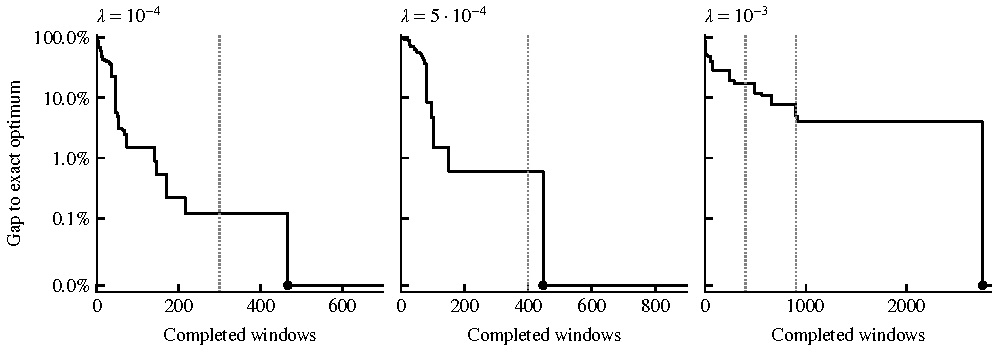
\includegraphics[width=\linewidth]{figures/portfolio-pce-progress.pdf}
\caption{Gap to the exact optimum during the three PCE chains.
Vertical dotted lines mark continuation runs, and filled dots mark the first attainment of the optimum.
The gap axis is logarithmic above 0.1\% and linear near zero.}
\label{fig:pce}
\end{figure}

The three optima first appeared after 467, 447, and 2,752 completed windows, respectively.
The corresponding circuit counts were 149,907, 143,487, and 883,392.
Figure~\ref{fig:pce} uses completed windows as its time axis because the JSON traces record rounded iteration
times and omit some setup costs. Continuing after discovery brought the total circuit counts to
224,700, 288,900, and 910,677.

A four-layer QAOA window search, initialized with Characterization Service angles, reached \(-68{,}249\)
at \(\lambda=10^{-4}\), 1.775\% above the optimum, using up to 18 qubits and 30,200 circuits.
Partitioned QAOA followed by repair reached \(-3{,}484\), then \(-54{,}923\) after classical local search.
On \texttt{po\_a010\_t10\_s02}, the best PCE result at \(\lambda=10^{-4}\) was \(-53{,}220\),
35 units above the exact optimum of \(-53{,}255\).

\clearpage
\section{Verification, interpretation, and reproduction}

The benchmark scorer recomputes each objective from the holdings in its solution file.
We independently rescored all 112 new classical files with published references.
The archived verification log records successful feasibility and score checks for all 125 files using the
notebook's Python implementation of the QOBLIB referee.
The earlier audit in \path{deliverables/portfolio/audit.csv} records the source files, method settings, and
objective checks for the pool-and-LNS, exact-DP, and quantum experiments.

The fifty-asset record scores come from classical methods. At \(\lambda=10^{-2}\) on
\texttt{po\_a050\_t10\_s00}, three exploratory PCE runs from empty holdings ended at \(-1000\).
A further 600-window run from the earlier classical \(-17{,}675\) solution also retained its starting score.
The three PCE optimum matches on ten assets show that small simulated circuits can produce improving window
assignments. A comparison with a classical conditional-QUBO solver at a common budget would help quantify
the contribution of PCE, including circuit evaluation, parameter optimization, repair, and scoring.

The new search is implemented in \path{portfolio_search.py}. Its archived traces, campaign settings, and
verification output are under \path{ai_context/portfolio_classical/}.
The earlier pool-and-LNS solver, exact DP, and conditional quantum search are in \path{portfolio_QIcing/},
along with their run logs. The following commands verify the new classical files and rebuild both report figures
from the repository root with the Python environment active.
\begin{verbatim}
PORTFOLIO_SOL_DIR=deliverables/portfolio python portfolio_search.py verify
python -m ai_context.scripts.plot_portfolio_report
\end{verbatim}

\begin{thebibliography}{9}
\bibitem{qoblib}
QOBLIB.
\href{https://github.com/ZIB-AOPT/QOBLIB/tree/main/06-portfolio}{Portfolio optimization benchmark},
model, checker, and published reference objectives.

\bibitem{pce}
M. Sciorilli et al.
\href{https://doi.org/10.1038/s41467-024-55346-z}{Towards large-scale quantum optimization solvers with few qubits}.
\emph{Nature Communications}, 16, 476, 2025.
\end{thebibliography}
\end{document}
